%%%%%%%%%%%%
%% Please rename this main.tex file and the output PDF to
%% [lastname_firstname_graduationyear]
%% before submission.
%%%%%%%%%%%%

\documentclass[12pt]{caltech_thesis}
\usepackage[hyphens]{url}
\usepackage{lipsum}
\usepackage{graphicx}
\usepackage{xcolor}

%\usepackage{todonotes}

%% Tentative: newtx for better-looking Times
\usepackage[utf8]{inputenc}
\usepackage[T1]{fontenc}
\usepackage{newtxtext,newtxmath}

% Must use biblatex to produce the Published Contents and Contributions, per-chapter bibliography (if desired), etc.
\usepackage[
    backend=biber,natbib,
    %backend=natbib,
    % IMPORTANT: load a style suitable for your discipline
    style=authoryear-comp,
    doi=False,
    bibstyle=apj
]{biblatex}
\renewcommand*{\nameyeardelim}{\addspace}
%\usepackage{natbib}
%\bibliographystyle{apj}
\newcommand{\todo}[3]{{\color{#2} \emph{#1} TO DO: #3}}
\newcommand{\btmtodo}[1]{\todo{BEN}{red}{#1}}

\renewcommand{\d}[1]{\ensuremath{\operatorname{d}\!{#1}}}


% Name of your .bib file(s)
\addbibresource{exopapers.bib}
\addbibresource{example.bib}

\begin{document}

% Do remember to remove the square bracket!
\title{Low-Mass Stars and Their Companions}
\author{Benjamin Tyler Montet}

\degreeaward{Doctor of Philosophy}                 % Degree to be awarded
\university{California Institute of Technology}    % Institution name
\address{Pasadena, California}                     % Institution address
\unilogo{caltechseal2.png}                                 % Institution logo
\copyyear{2017}  % Year (of graduation) on diploma
\defenddate{July 18, 2016}          % Date of defense

\orcid{0000-0001-7516-8308}

%% IMPORTANT: Select ONE of the rights statement below.
%\rightsstatement{All rights reserved\todo[size=\footnotesize]{Choose one from the choices in the source code!! And delete this \texttt{todo} when you're done that. :-)}}
 \rightsstatement{All rights reserved except where otherwise noted}
% \rightsstatement{Some rights reserved. This thesis is distributed under a [name license, e.g., ``Creative Commons Attribution-NonCommercial-ShareAlike License'']}

%%  If you'd like to remove the Caltech logo from your title page, simply remove the "[logo]" text from the maketitle command
\maketitle[logo]
%\maketitle

\begin{acknowledgements} 	 
   People to thank: John + group. Brendan Bowler, Justin, Luan, 
   Hogg, DFM, Ruth. 
   Ian, Dawn, Ryan, Jieun, Aaron and Jason
   Cahill department and traditions - see Sirio's.
   Antonija + Mislav, Trevor, Allison, Yi. Matt, Sirio, Gwen and Drew, Ryan.
   Committee, Patrick and Anu
   Laura
   Parents
   
\end{acknowledgements}

\begin{abstract}
   [This abstract must provide a succinct and informative condensation of your work. Candidates are welcome to prepare a lengthier abstract for inclusion in the dissertation, and provide a shorter one in the CaltechTHESIS record.]
\end{abstract}

%% Uncomment the `iknowhattodo' option to dismiss the instruction in the PDF.
%\begin{publishedcontent}%[iknowwhattodo]
% List your publications and contributions here.
%\nocite{Cahn:etal:2015}
%\end{publishedcontent}

\tableofcontents
\listoffigures
\listoftables
%\printnomenclature

\mainmatter

\chapter{Introduction}

\section{M Dwarfs: The Silent Majority}
For much of the timescale of stellar astrophysics research, to a fanatic 
of M dwarf stars their history is a story of neglect and underappreciation.
The first spectrum of an M dwarf was obtained only 100 years ago when 
\citet{Adams13} collected an observation of the M+M binary Groombridge 34.
The oldest known surviving diagram plotting stellar absolute magnitude against spectral type \citep{Russell14}, now known as a Hertsprung-Russell Diagram, includes hundreds of stars, as shown in Figure \ref{fig:HR}.
Today we know that M dwarfs make up approximately 75\% of the stars in the galaxy,
yet only $\sim$5\% of the stars included in Russell's figure are listed as
spectral type M.



\begin{figure}[hbt!]
\centering
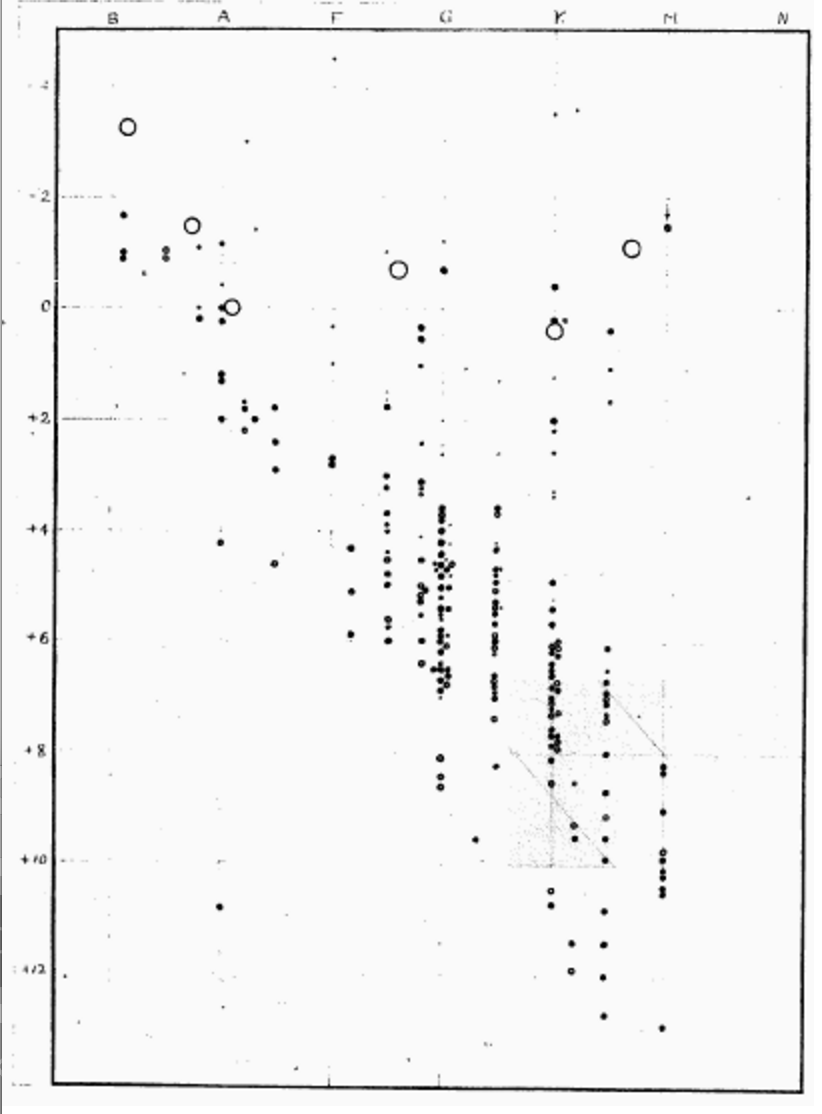
\includegraphics[width=.5\textwidth]{hr.png}
\caption{\btmtodo{This is a figure}}
\label{fig:HR}
\index{Example Figure}
\end{figure}

Russell and others hold no personal grudge against M dwarfs, the prolem is the physics
of M dwarfs themselves.
To show this, let us begin with the equations of stellar structure.
The first of these declares a star is in hydrostatic equilibrium:
\begin{equation}
\frac{\d P(r)}{\d r} = - \frac{ G m \rho}{r^2 },
\label{eq:hydro}
\end{equation}
where $P(r)$ is the pressure exerted on a particle at a radius $r$, $G$ is Newton's
constant, $m$ the mass enclosed inside the radius $r$, and $\rho$ the stellar density,
itself a function of radius as well.

The second equation defines mass conservation:
\begin{equation}
\frac{\d m(r)}{\d r} = 4 \pi r^2 \rho,
\end{equation}
where $\pi$ is the ratio of a circle's circumference to its diameter,
and all other variables retain their meaning from Equation \ref{eq:hydro}.

The third equation defines energy transport:
\begin{equation}
\frac{\d L(r)}{\d r} = 4 \pi r^2 \rho \epsilon,
\end{equation}
where $L$ is the energy leaving a spherical shell of radius $r$, produced by the
material in the star interior to $r$ and $\epsilon$ is the energy released per unit
mass per second inside the star.

The final equation defines the temperature gradient inside a star. 
The exact form of this equation depends on the method for which energy is transported
inside the star.
For radiative transport, the temperature gradient is
\begin{equation}
\frac{\d T}{\d r} = - \frac{3}{4ac} \frac{\bar{\kappa} \rho}{T^3} \frac{L}{4\pi r^2}.
\end{equation}
Here, $T$ is the temperature of the star at a radius $r$, $ac$ is the radiation constant multiplied by the speed of light, also equal to four times the Stefan-Boltzmann
constant, and $\bar{\kappa}$ the mean opacity of the material.

Very low-mass stars are fully convective, not radiative, and therefore follow
a different limit:
\begin{equation}
\frac{\d T}{\d r} =  \bigg( 1 - \frac{1}{\gamma}\bigg)\frac{T}{P}\frac{\d P(r)}{\d r},
\end{equation}
where $\gamma$ is the adiabatic index, and is $5/3$ for a monatomic ideal gas,
and all other terms retain their previous meaning.

Let us consider two other proportionalities. First, we assume that the energy generation rate
inside a star is a function of its temperature and density:
\begin{equation}
\epsilon = \epsilon_0 \rho T^\nu
\end{equation}
where $\nu$ depends on the particular fusion pathway that is dominant in the core of
the star.
Second, we assume that the ideal gas law holds:
\begin{equation}
P \propto \rho T.
\end{equation}

With these six equations, we can develop a series of homology relations. We can create
a series of five linear equations with five unknown parameters: $\log T$, $\log P$, 
$\log R$, $\log \rho$, and $\log M$.
Ignoring constant terms and considering only the adiabatic case (as for fully 
convective stars),
\begin{align}
\log P &= 2 \log M - 4 \log R \nonumber \\
\log \rho &= \log M - 3 \log R \nonumber \\
\log P &= \gamma \log \rho \\
\log T &= \bigg(\frac{\gamma - 1}{\gamma}\bigg) \log P \nonumber \\
\log L &= \log \rho + \nu \log T + \log M \nonumber.
\end{align}
We can rearrange these to solve for $\log M$, finding
\begin{equation}
\log R = \bigg(\frac{2-\gamma}{4 - 3\gamma}\bigg) \log M,
\end{equation}
which we can then insert into the final equation in Equation 1.8.
This manipulation yields
\begin{equation}
\log L = \bigg(\frac{2(\nu + 1) - \gamma(2\nu + 3)}{4 - 3\gamma}\bigg) \log M,
\end{equation}
which if we consider the case where we have an ideal, fully ionized gas so that $\gamma = 5/3$ and energy generation dominated by the p-p chain so that $\nu = 4$, we find
\begin{equation}
\log L \approx 8.33 \log M
\end{equation}
or $L \propto M^{8.33}$! Thus, if we decrease the mass of a fully convective star by a factor of two, 
we also decrease its luminosity by a factor of 320!\footnote{The same manipulation,
considering the case of radiative transport, leads to the relation $L~\propto~M^{5.5}$,
similar to what is observed for Sun-like stars.} 

Even worse for optical observing,
the peak of the SED of a typical 3,000 K M dwarf peaks at 1 micron, well into the infrared, making them even fainter in the optical.
Even though M dwarfs make up 70\% of the nearest stars, with 250 of them located within
10 pc of the Sun \citep[e.g.][]{Henry06}, there are no M dwarfs visible to the naked 
eye.
The brighest, HIP\,105090, is only $3.95 \pm 0.01$ pc from the Sun, yet has an apparent V-band magnitude of 6.76 \citep{vanLeeuwen07}.
With so many bright solar-type stars in the solar neighborhood, it is easy to understand why M dwarfs have been and often continue to be overlooked in planet search
surveys. 

\section{Radial Velocity Planet Searches}
The first radial velocity (RV) planet searches focused almost exclusively on Sunlike
(FGK) stars. 
There are two biases that make this a reasonable choice of star. 
First, 

FGK are good
found a bunch of new planets
why change?

Slowly moved into searches for planets around other types of stars
John's subgiants
M dwarf searches---CPS and HARPS
Didn't find so many

RV limitations: large planets, close in.
Can't find very small planets, or very distant ones
what's the best place to search? Mike Bottom's paper.

Planets in wide orbits: motivate TRENDS survey.

\section{Transiting Planets}


\section{Understanding M Dwarfs}
One of the other downsides of studying companions to M dwarfs is the difficulty 
in inferring stellar parameters.

\btmtodo{Transit, RV planet params from stellar params}
\btmtodo{Where are we as a field in M dwarf params? Much closer than 5 years ago
but still not great}

\btmtodo{Talk about M+M binaries here}

\section{Brown Dwarfs}
\btmtodo{Say something about irradiation here---M dwarfs are nice!}

\section{Goals of this Thesis} 

\btmtodo{See Drew's thesis for tips on formatting previous papers section}


Start off all chapters with \verb|chapter|. \index{chapter!numbered} \verb|\extrachapter| will give you an unnumbered chapter that's added to the Table of Contents. \index{chapter!unnumbered}

Here's an example of a citation \citep{GMP81}. Here's another \citep{PP98}. These will appear in the big bibliography at the end of the thesis.
\index{bibliography}

If you're new to \LaTeX{} and would like to begin by learning the basics, please see our free online course available at:\\ \url{https://www.overleaf.com/latex/learn/free-online-introduction-to-latex-part-1} \index{LaTeX@\LaTeX}

You can define nomenclatures \index{nomenclature} as you talk about key terms in your thesis. So what's a galaxy? %\nomenclature{Galaxy}{A system of stars independent from all other systems}


\section{This is a Section}
\lipsum[1-2]

\begin{figure}[hbt!]
\centering

\includegraphics[width=.3\textwidth]{caltech.png}
\caption{This is a figure}\label{fig:logo}
\index{Example Figure}
\end{figure}

\subsection{This is a subsection}

\begin{table}[hbt!]
\centering
\begin{tabular}{ll}
\hline
Area & Count\\
\hline
North & 100\\
South & 200\\
East & 80\\
West & 140\\
\hline
\end{tabular}
\caption{This is a table}\label{tab:sample}
\index{tables}
\end{table}

\lipsum[3] \nomenclature{Asteroid}{A very small planet ranging from 1,000 km to less than one km in diameter. Asteroids are found commonly around other larger planets}

\lipsum[4-5] 

Here's an endnote.\endnote{Endnotes are notes that you can use to explain text in a document.}

\section{This is Another Section}
\lipsum[6-7] 

\chapter{This is the Second Chapter}
%\begin{refsection}
%If you'd like to have separate bibliographies at the end of each chapter, %put a \verb|refsection| around the material of each chapter, then cite as usual -- e.g.~\citep{GMP81,Ful83}. Then do a \verb|\printbibliography| just before the \verb|refsection| ends. \index{bibliography!by chapter}

%\printbibliography[heading=subbibliography]
%\end{refsection}
\btmtodo{This is the Dynamical Masses TTV paper}


\chapter{This is the Third Chapter}

%\publishedas{Cahn:etal:2015}

[You can have chapters that were published as part of your thesis. The text style of the body should be single column, as it was submitted to the publisher, not formatted as the publisher did.]

\btmtodo{This is TRENDS IV}

\chapter{This is the Fourth Chapter}

\btmtodo{This is LHS Part 1}
\chapter{This is the Fifth Chapter}

\btmtodo{This is LHS Part II}

\chapter{This is the Sixth Chapter}

\btmtodo{This is the M+M binary work}

\chapter{This is the Seventh Chapter}

\btmtodo{This is the K2 planet catalog}

\chapter{This is the Eighth Chapter}

\btmtodo{This is WFIRST}

\chapter{This is the Ninth Chapter}

\btmtodo{This is the summary and future directions}

\printbibliography[heading=bibintoc]
%\bibliography{exopapers}

%\appendix

%\chapter{Questionnaire}
%\chapter{Consent Form}

%\printindex

%\theendnotes

%% Pocket materials at the VERY END of thesis
%\pocketmaterial
%\extrachapter{Pocket Material: Map of Case Study Solar Systems} 


\end{document}

